\subsection{Partitioneren van geheugen}

Partitioneren is een van de eerste methodes voor het beheren van geheugen. Het virtuele geheugen is geëvolueerd van partitionering methodes.

Soorten partitionering:


\begin{itemize}
\item Vaste partitionering
\item Dynamische partitionering
\item Eenvoudige paginering
\item Eenvoudige segmentatie
\item Paginering met virtueel geheugen
\item Virtual-Memory segmentatie
\end{itemize}

\subsubsection{Vaste partitionering}

Bij de meeste vormen voor geheugenbeheer mogen we aannemen dat het besturingssysteem een vast deel van het hoofdgeheugen bezet en dat de rest van het hoofdgeheugen beschikbaar is voor gebruik door meerdere processen.

Partities met een vaste grootte kennen twee problemen:
	
\begin{itemize}
\item Een programma kan te groot zijn om in een partitie te passen. Dan moet de programmeur het programma ontwerpen dat overlays gebruikt, zodat altijd maar een deel van het programma zich in het hoofdgeheugen hoeft te bevinden. Is er een module nodig die nog niet aanwezig is, dan moet het gebruikersprogramma dit in de partitie van het programma laden en de programma’s of gegevens die zich daar bevinden vervangen.
\item Er is een inefficiënt gebruik van het geheugen: Elk proces hoe klein ook, bezet meteen 
een hele partitie
\end{itemize}
=> interne fragmentatie

Bij gebruik van Partities van ongelijke grootte is er minder interne fragmentatie.

Bij Partities van gelijke grootte speelt de plaatsing van processen nauwelijks een rol. Zolang maar een partitie beschikbaar is, kan een proces in die partitie geplaatst worden.

Bij Partities met een ongelijke grootte kan:

\begin{itemize}
    \item Men een proces vast toewijzen aan de kleinste partitie waar het in past. Elke partitie heeft een wachtrij en processen.
        \begin{itemize}
        \item Voordeel: er is een minimalisatie van interne fragmentatie
        \end{itemize}
    \item Men gebruik maken van 1 wachtrij: als er bvb een proces van < 8mb ingeroosterd moet worden en de Partities van 8 mb zijn op, dan zal er niet gewacht worden maar het proces zal worden geplaatst in een partitie van een grotere grootte.
\end{itemize}

\subsubsection{Dynamische indeling van partities}

Bij dynamisch Partitioneren wordt een variabel aantal Partities van variabele grootte gebruikt. $\Rightarrow$ wordt een proces overgebracht naar het geheugen, dan krijgt het de hoeveelheid geheugen dat het nodig heeft en niet meer.

Nadeel: na verloop van tijd ontstaan er vele kleine gaten in het geheugen die elk apart te klein zijn om een proces te kunnen bevatten: externe fragmentatie: het geheugen wordt buiten de partities gefragmenteerd $\leftrightarrow$ interne fragmentatie: binnen de partities zelf.

Een oplossing voor deze externe fragmentatie is compaction: van tijd tot tijd worden de processen herschoven binnen het geheugen zodat ze aaneengesloten zijn en al het vrije geheugen 1 blok vormt.

Er is wel een nadeel: compaction is verspilling van veel processortijd. Een vereiste voor compaction is dynamische Relocatie: het moet mogelijk zijn een programma te verplaatsen van het ene naar het andere gebied zonder de geheugenverwijzingen in het programma ongeldig te maken.

Plaatsingsalgoritmes:

\begin{itemize}
    \item Best-fit
        \begin{itemize}
        \item Het toewijzen van een zo klein mogelijke, niet-bezet blok geheugen aan een proces.
        \end{itemize}
    \item First-fit
    \begin{itemize}
        \item Doorzoekt het geheugen vanaf het begin en wijst het eerste niet-bezette blok toe aan een proces. Dit werkt het snelst.
        \end{itemize}
    \item Next-fit
    \begin{itemize}
        \item Doorzoekt het geheugen vanaf de plaats waar de laatste plaatsing is gebeurd en wijst het volgende beschikbare blok toe dat groot genoeg is. Dit algoritme zal vaker geheugen toewijzen dat zich aan het einde van het geheugen bevindt.
        \end{itemize}
\end{itemize}

Nadelen per strategie:

\begin{itemize}
    \item Best-fit
        \begin{itemize}
        \item geheugencompactie moet vaker gebeuren dan bij de andere algoritmes:
        \item hoofdgeheugen raakt veel sneller vervuild met kleine blokken vrij geheugen die niet bruikbaar zijn om processen aan toe te wijzen $\Rightarrow$ best-fit presteert het slechtst.
        \end{itemize}
    \item First-fit
    \begin{itemize}
        \item het voorste deel van het geheugen gaat snel volzitten met kleine blokken die té klein zijn voor processen. Het probleem is dat deze toch worden doorzocht bij aanvang van het algoritme
        \end{itemize}
    \item Next-fit
    \begin{itemize}
        \item het grootste blok vrije geheugen (einde van het geheugen) wordt vrij snel opgesplitst in kleine delen => compaction zal vaker nodig zijn
        \end{itemize}
\end{itemize}



\subsubsection{Buddysysteem}

Zowel vaste als dynamische partitionering hebben nadelen:

\begin{itemize}
\item vast: beperkt het aantal actieve processen en inefficiënt geheugengebruik.
\item dynamisch: veel onderhoud en overhead door compaction
\end{itemize}


Volledig beschikbare ruimte = $2^u$

Wanneer nu een proces moet worden toegewezen aan geheugen, dan wordt gecontroleerd of 2u-1 < s <=2u Als dat zo is, dan wordt het hele geheugenblok toegewezen aan het proces.

Als dat niet zo is, dan wordt het blok opgedeeld in twee gelijke 'buddies' en het opnieuw gecontroleerd totdat dit zo is en het proces kan worden toegewezen.

Het buddysysteem omzeilt de problemen van vaste en dynamische partitionering MAAR het virtueel geheugen, gebaseerd op pagineren en segmenteren is veel beter.

\subsubsection{Relocatie}

Wanneer een programma in het geheugen wordt geladen worden de echte (absolute) geheugenlocaties bepaald.

Een proces kan verschillende partities bevatten wat betekent dat er met verschillende absolute geheugenlocaties moet gewerkt worden tijdens de uitvoering van het proces.

Elk relatief adres ondergaat twee bewerkingen in de processor:

\begin{enumerate}
\item Eerst wordt de waarde van het basisregister opgeteld bij het relatief adres om een absoluut adres te krijgen (beginadres + relatief adres = absoluut adres)
\item Dat absoluut adres wordt vergeleken met het adres in het grensregister $\Rightarrow$ ligt het verkregen adres niet tussen de grenzen $\Rightarrow$ er wordt een interrupt gegenereerd naar het OS dat moet reageren op deze fout. Ligt het wel tussen de grenzen, dan mag er verdergegaan worden met de uitvoering van de instructie
\end{enumerate}

\begin{figure}[htp]
    \centering
            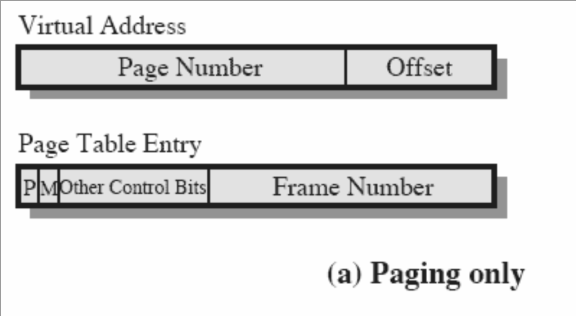
\includegraphics[width=4in]{img/pagineren.png}
        \caption{Paging only}
    \label{fig:Paging only}
\end{figure}